% +++++++++++++++++++++++++++++++++++++++++++++++++++++++++++
% University of Southern Maine
% Department of Computer Science
% Discrete Mathematics II (COS 280)
% James Quinlan (https://cs.usm.maine.edu/~james.quinlan/)
% Homework Template
% +++++++++++++++++++++++++++++++++++++++++++++++++++++++++++


% EDIT Lines: 11, 12, 13
\def\filename{Dynamic Programming}   		   % included file (edit file)
\def\chapsec{Chapter 3}  % Chapter/Section/Topic
\def\yourname{Dynamic Programming}	   % Your name
\def\course{COS 485}		   % Course (if different)



% ---------------- Do NOT Edit Below ------------------------
% -----------------------------------------------------------
\documentclass[11pt]{article}

\def\pf{\textit{Proof}: }

\usepackage{mathtools}
\usepackage{epsfig}
\usepackage{amsfonts}
\usepackage{amssymb}
\usepackage{amstext}
\usepackage{amscd}
\usepackage{amsmath}
\usepackage{xspace}
\usepackage{theorem}
\usepackage{float}
\usepackage[table]{xcolor}
\usepackage{color}
\usepackage{soul}
\usepackage{booktabs}
\usepackage{outlines}
\usepackage{enumitem}
\usepackage{algorithm}
\usepackage{algpseudocode}
\usepackage{pgf-pie}
\usepackage{fancybox}
\usepackage{circuitikz}
\setenumerate[1]{label=\arabic*.}
\setenumerate[2]{label=(\alph*).}
\setenumerate[3]{label=\roman*.}
\setenumerate[4]{label=\alph*.}

\usepackage{hyperref}
\hypersetup{
    colorlinks=true,
    linkcolor=blue,
    filecolor=magenta,      
    urlcolor=cyan,
    pdftitle={\filename},
    pdfpagemode=FullScreen,
    }

% TikZ
\usepackage{tikz}
\usepackage{pgfplots}
\pgfplotsset{compat=1.15}
\usepackage{mathrsfs}
\usetikzlibrary{arrows}

% Colors
\definecolor{stainlessSteel}{cmyk}{0,0,0.02,0.12}

% Document Geometry
\makeatletter
 \setlength{\textwidth}{6.75in}
 \setlength{\oddsidemargin}{0in}
 \setlength{\evensidemargin}{0in}
 \setlength{\topmargin}{0.0125in}
 \setlength{\textheight}{9.0in}
 \setlength{\headheight}{0pt}
 \setlength{\headsep}{0pt}
 \setlength{\marginparwidth}{59pt}

 \setlength{\parindent}{0pt}
 \setlength{\parskip}{5pt plus 1pt}
 \setlength{\theorempreskipamount}{5pt plus 1pt}
 \setlength{\theorempostskipamount}{0pt}
 \setlength{\abovedisplayskip}{8pt plus 3pt minus 6pt}
 \setlength{\intextsep}{15pt plus 3pt minus 6pt}

 % Headings
 \renewcommand{\section}{\@startsection{section}{1}{0mm}%
    {2ex plus -1ex minus -.2ex}%
    {1.3ex plus .2ex}%
    {\normalfont\Large\bfseries}}%
 \renewcommand{\subsection}{\@startsection{subsection}{2}{0mm}%
    {1ex plus -1ex minus -.2ex}%
    {1ex plus .2ex}%
    {\normalfont\large\bfseries}}%
 \renewcommand{\subsubsection}{\@startsection{subsubsection}{3}{0mm}%
    {1ex plus -1ex minus -.2ex}%
    {1ex plus .2ex}%
    {\normalfont\normalsize\bfseries}}
 \renewcommand\paragraph{\@startsection{paragraph}{4}{0mm}%
    {1ex \@plus1ex \@minus.2ex}%
    {-1em}%
    {\normalfont\normalsize\bfseries}}
 \renewcommand\subparagraph{\@startsection{subparagraph}{5}{\parindent}%
    {2.0ex \@plus1ex \@minus .2ex}%
    {-1em}%
    {\normalfont\normalsize\bfseries}}
\makeatother

\newcounter{thelecture}

\newenvironment{proof}{{\bf Proof:  }}{\hfill\rule{2mm}{2mm}}
\newenvironment{proofof}[1]{{\bf Proof of #1:  }}{\hfill\rule{2mm}{2mm}}
\newenvironment{proofofnobox}[1]{{\bf#1:  }}{}
\newenvironment{example}{{\bf Example: }}{\hfill\rule{0mm}{0mm}} % change 2mm 2mm for square

%\renewcommand{\theequation}{\thesection.\arabic{equation}}
%\renewcommand{\thefigure}{\thesection.\arabic{figure}}

\newtheorem{fact}{Fact}
\newtheorem{lemma}[fact]{Lemma}
\newtheorem{theorem}[fact]{Theorem}
\newtheorem{definition}[fact]{Definition}
\newtheorem{corollary}[fact]{Corollary}
\newtheorem{proposition}[fact]{Proposition}
\newtheorem{claim}[fact]{Claim}
\newtheorem{exercise}[fact]{Exercise}

% math notation
\newcommand{\R}{\ensuremath{\mathbb R}}
\newcommand{\Z}{\ensuremath{\mathbb Z}}
\newcommand{\N}{\ensuremath{\mathbb N}}
\newcommand{\B}{\ensuremath{\mathbb B}}
\newcommand{\F}{\ensuremath{\mathcal F}}
\newcommand{\SymGrp}{\ensuremath{\mathfrak S}}
\newcommand{\prob}[1]{\ensuremath{\text{{\bf Pr}$\left[#1\right]$}}}
\newcommand{\expct}[1]{\ensuremath{\text{{\bf E}$\left[#1\right]$}}}
\newcommand{\size}[1]{\ensuremath{\left|#1\right|}}
\newcommand{\ceil}[1]{\ensuremath{\left\lceil#1\right\rceil}}
\newcommand{\floor}[1]{\ensuremath{\left\lfloor#1\right\rfloor}}
\newcommand{\ang}[1]{\ensuremath{\langle{#1}\rangle}}
\newcommand{\poly}{\operatorname{poly}}
\newcommand{\polylog}{\operatorname{polylog}}

% Anupam's abbreviations
\newcommand{\e}{\epsilon}
\newcommand{\half}{\ensuremath{\frac{1}{2}}}
\newcommand{\junk}[1]{}
\newcommand{\sse}{\subseteq}
\newcommand{\union}{\cup}
\newcommand{\meet}{\wedge}
\newcommand{\dist}[1]{\|{#1}\|_{\text{dist}}}
\newcommand{\hooklongrightarrow}{\lhook\joinrel\longrightarrow}
\newcommand{\embeds}[1]{\;\lhook\joinrel\xrightarrow{#1}\;}
\newcommand{\mnote}[1]{\normalmarginpar \marginpar{\tiny #1}}



% -----------------------------------------------------------
% Header
\newcommand{\hwheadings}[3]{
{\chapsec } \hfill {{ \yourname }} \hfill {{ \course #1}}\\
{{\bf } #2} \hfill { #3} 
\rule[0.051in]{\textwidth}{0.0025in}
%\thispagestyle{empty}
}

% Document begins here 
\begin{document}
\hwheadings{}{}{}
\section*{\centering Dynamic Programming}
\label{sec:dynamic-programmiung}

\section*{Overview}

\begin{outline}[enumerate]
  \1 Background
  \1 Framework 
  \1 Examples 
\end{outline}

\section*{Background}%
\label{sec:background}

Dyanmic Programming (DP) applies to \textbf{optimization} problems. It is used to solve many problems in 
polynomial time. $O(n^c)$  \textbf{instead} of $O(c^n)$. To use Dynamic Programming, a problem must have
\begin{itemize}
  \item Overlapping Subproblems 
\end{itemize}

\begin{figure}[!ht]
\centering
% EDIT FOR PICTURE SIZING
\resizebox{3cm}{!}{%
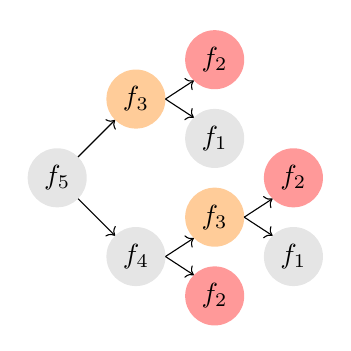
\begin{tikzpicture}

  %Styles for picture
  \tikzset
  {
  vertex/.style={circle, inner sep=0pt, outer sep=0pt, minimum width=0.75cm,fill=black!10},
  redvertex/.style={circle, inner sep=0pt, outer sep = 0pt, minimum width = 0.75cm, fill=red!40}, 
  orangevertex/.style={circle, inner sep=0pt, outer sep = 0pt, minimum width = 0.75cm, fill=orange!40}, 
  }

  %Nodes
  \node[vertex] (v1) at (1,3) {$f_5$};
  \node[orangevertex] (v2) at (2,4) {$f_3$};
  \node[vertex] (v3) at (2,2) {$f_4$};
  \node[orangevertex] (v4) at (3,2.5) {$f_3$};
  \node[redvertex] (v5) at (3,1.5) {$f_2$};
  \node[redvertex] (v6) at (3,4.5) {$f_2$};
  \node[vertex] (v7) at (3,3.5) {$f_1$};
  \node[redvertex] (v8) at (4,3) {$f_2$};
  \node[vertex] (v9) at (4,2) {$f_1$};
  

  %Edges
  \draw[->] (v1.north east) -- (v2.south west);
  \draw[->] (v1.south east) -- (v3.north west);
  \draw[->] (v2.east) -- (v6.south west);
  \draw[->] (v2.east) -- (v7.north west);
  \draw[->] (v3.east) -- (v4.south west);
  \draw[->] (v3.east) -- (v5.north west);
  \draw[->] (v4.east) -- (v8.south west);
  \draw[->] (v4.east) -- (v9.north west);
\end{tikzpicture}
}%
\label{fig:subproblems}
\end{figure}

Divide and Conquer is very innefficient when the `smaller' problem is nearly as large as the original.
DP is similar but smaller problems are solved first and then stored for later use.

\begin{itemize}
  \item Optimal Substructure
\end{itemize}

Optimal Substructure is a powerful principle that says the optimal solution of a bigger problem 
can be created from the optimal solutions of its smaller subproblems. It allows 
us to break a difficult problem into small manageable parts, and 
combine the results of these small problems to get the best solution to the overall problem.


\begin{figure}[!ht]
\centering
% EDIT FOR PICTURE SIZING
\resizebox{6cm}{!}{%
\begin{circuitikz}
% Oval and lines
\draw  (4.75,13.25) ellipse (5.5cm and 3cm);
\draw [short] (0.75,15.25) -- (1.75,10.75);
\draw [short] (4,16.25) -- (3.75,10.25);
\draw [short] (8.5,15.5) -- (8.5,11);

\node [font=\Huge] at (0.25,13) {$x_1$};
\node [font=\Huge] at (2.5,14.25) {$x_2$};
\node [font=\Huge] at (6.25,13.5) {...};
\node [font=\Huge] at (9.5,13.25) {$x_k$};

% Arrows
\draw [->, >=Stealth, dashed] (0.75,13) -- (2.25,14);
\draw [->, >=Stealth, dashed] (3,14) -- (5.5,13.5);
\draw [->, >=Stealth, dashed] (7,13.5) -- (9,13.25);

\end{circuitikz}
}%
\label{fig:substructure}
\end{figure}
\section*{Framework}%
\label{sec:framework}

\begin{outline}[enumerate]
  \1 Define the objective function
  \1 Identify the Base cases (Starting points)
  \1 Recurrence Relation. Subproblem $\Rightarrow$ Problem
  \1 Order of computation.
  \1 Location of the answer, F(n).
\end{outline}

The staircase problem is a classic example for the application of Dynamic Programming. \\
\textbf{Problem}: You are climbing a staircase. It takes $n$ steps to reach the top. Each time you 
can either climb 1 or 2 steps. In how many distinct ways can you climb to the top?

\begin{outline}[enumerate]
  \1 Objective Function
    \2 f(n) = the number of distinct ways to reach the $n^{th}$ step.
  \1 Base cases
    \2 $f(0) = 1$, as there is only one way to take no steps.
    \2 $f(1) = 1$, as there is only one way to take one step.
    \2  $f(2) = 2$, as you can either take two single steps, or one double step
  \1 Recurrence Relation
    \2 $f(n) = f(n-1) + f(n-2)$
  \1 Order of computation
    \2 Bottom-up
  \1 Location of the answer
    \2 Where to look - $f(n)$.
    \2 Time complexity -  $O(n)$
    \2 Space -  $O(n)$
\end{outline}

The bottom-up approach is being used as each value requires the previous two values to be found.
Instead of recomputing them every time like we would with a top-down approach, we can store the previous
values. This technique of storing previous values to find the next is called \textbf{Memoization}.


\begin{figure}[!ht]
\centering
% EDIT FOR PICTURE SIZING
\resizebox{8cm}{!}{%
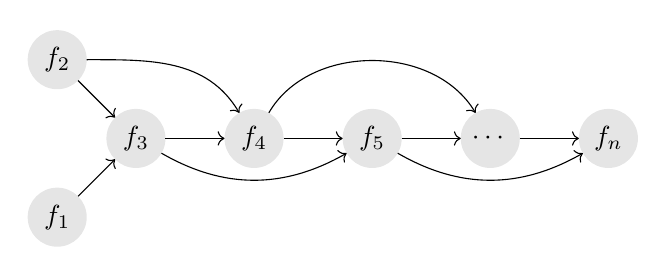
\begin{tikzpicture}

  %Styles for picture
  \tikzset
  {
  vertex/.style={circle, inner sep=0pt, outer sep=0pt, minimum width=0.75cm,fill=black!10},
  redvertex/.style={circle, inner sep=0pt, outer sep = 0pt, minimum width = 0.75cm, fill=red!40}, 
  orangevertex/.style={circle, inner sep=0pt, outer sep = 0pt, minimum width = 0.75cm, fill=orange!40}, 
  }
  
  % Nodes
  \node[vertex] (v1) at (0,3) {$f_1$};
  \node[vertex] (v2) at (0,5) {$f_2$};
  \node[vertex] (v3) at (1,4) {$f_3$};
  \node[vertex] (v4) at (2.5,4) {$f_4$};
  \node[vertex] (v5) at (4,4) {$f_5$};
  \node[vertex] (v6) at (5.5,4) {$\cdots$};
  \node[vertex] (v7) at (7,4) {$f_{n}$};

  % Edges
  \draw[->] (v1) -- (v3);
  \draw[->] (v2) -- (v3);
  \draw[->] (v3) -- (v4);
  \draw[->] (v2) to [out=0, in=120] (v4); % bendy
  \draw[->] (v4) -- (v5);
  \draw[->] (v3) to [out=330, in=210] (v5); % bendy
  \draw[->] (v5) -- (v6);
  \draw[->] (v4) to [out=60, in=120] (v6); % bendy
  \draw[->] (v6) -- (v7);
  \draw[->] (v5) to [out=330, in=210] (v7); % bendy
\label{fig:bottom-up}
\end{tikzpicture}
}%
\end{figure}

\section*{Examples}%
\label{sec:examples}

\subsection*{Fibonacci Sequence}%
\label{sub:fibonacci}

Consider the fibonacci sequence, where the two previous numbers in the sequence are used to calculate the next number.
\[
  1 + 1 = 2 + 1 = 3 + 2 = 5 + 3 = 8 + 5 = 13 \cdots 
\]

The Problem: Given a number $n$, find the  $n^{th}$ term in the fibonacci sequence.

This problem is a classic example of how applying dynamic-programming can make finding a solution go from 
factorial (binomial) time down to polynomial time.

\textbf{Recursive (Exponential Solution)}

As shown above, calculating the $n^{th}$ fibonacci number recursively is very innefficient.
Using the Recurrence Relation for it, we can solve for the explicit solution, and find the time complexity for 
the recursive algorithm

\begin{algorithm}
  \caption{Recursive Fibonacci}\label{alg:fib}
  \begin{algorithmic}
  \State \textbf{Input}
  \State $n \gets$ the $n^{th}$ term in the sequence
  \State \textbf{Function} fib(n) $\rightarrow x \in \Z$
  \If{$n \le 2$}
    \State \textbf{return} $1$;
  \Else
    \State \textbf{return} fib(n-1)  + fib(n-2);
  \EndIf
  \end{algorithmic}
\end{algorithm}

Since this reursive algorithm has one operation for every call of the function, 
it's operations can be quantified by the recurrence relation
\[
  T(n) = T(n-1) + T(n-2) \\ 
\] 
\begin{align*}
  & T(0) = 0 & T(1) = 1 & & T(2) = 1
\end{align*}

We can then rearrange mathematically to find the explicit solution, and time complexity for our 
recursive solution.

First rearrange into a Linear Homogenous Recurrence Relation with Constant Coefficients (LHRRCC)
\[
T(n) - T(n-2) - T(n-2) = 0
\] 
Then find the roots using the quadratic formula on the characteristic equation

\begin{align*}
  &x^2 - x^1 - 1 = 0 \\ 
  &x_{1} = \frac{1 + \sqrt{5}}{2} \\
  &x_{2} = \frac{1 - \sqrt{5}}{2}
\end{align*}

Then apply those roots to the General Solution Equation
\[
  f_{n} = Ax_{1}^n + Bx_{2}^n
\] 

Now solve for A and B

\begin{align*}
  f_{0} = 0 &= A(1) + B(1)
  &\therefore A = -B \\ 
  f_{1} = 1 &= A\left(\frac{1 + \sqrt{5}}{2}\right) + B\left(\frac{1 - \sqrt{5}}{2}\right) \\ 
  1 &= A\left(\frac{1 + \sqrt{5}}{2}\right) - A\left(\frac{1 + \sqrt{5}}{2}\right) \\
  A &= \frac{1}{5} \; \; B = -\frac{1}{5} 
\end{align*}

Which means the explicit solution is

\[
  T(n) = \frac{1}{5} \left(\frac{1 + \sqrt{5}}{2}\right)^n -\frac{1}{5}\left(\frac{1 - \sqrt{5}}{2}\right)^n
.\] 
This proves that the recursive approach is an exponential function. An upperbound for the 
function could be described as $O(2^n)$.

\textbf{Dynamic Programming Solution}

The Fibonacci sequence can be solved using dynamic programming (DP) because it has these
charaacteristics

\begin{itemize}
  \item Optimization Problem (Factorial time)
  \item Optimal Subproblem Structure (Overlapping subproblems).
\end{itemize}

\begin{figure}[!htbp]
\label{fig:merge-sort}
\centering
\resizebox{10cm}{!}{%
\begin{circuitikz}

% Array
\draw  (5,20) rectangle  node {$1$} (6,19);
\draw  (6,20) rectangle  node {$1$} (7,19);
\draw  (7,20) rectangle  node {$2$} (8,19);
\draw  (8,20) rectangle  node {$3$} (9,19);
\draw  (9,20) rectangle  node {$5$} (10,19);
\draw  (10,20) rectangle  node {$8$} (11,19);
\draw  (11,20) rectangle  node {$13$} (12,19);
\draw  (12,20) rectangle  node {$\cdots$} (13,19);
\end{circuitikz}
}%
\end{figure}

Instead of doing the work from the top-down, and repeating calculations, the previous values
should be stored so that future elements can access them instead of recalculating it.

This can be done using an array with the fibonacci sequence. Then, use the recursive definition
but instead of recalculating, access the array for the previous values.

\[
  arr[i] = arr[i-1] + arr[i-2];
\] 

\textbf{Note} The following solution uses an array to store previous values, which has a space complexity of
$O(n)$. However, the optimal solution can use constant space $O(1)$ if only the previous two values were stored
with a \textit{Sliding Window} technique. \\

\begin{algorithm}
  \caption{Dynamic Programming Fibonacci}\label{alg:fib2}
  \begin{algorithmic}
  \State \textbf{Input}
  \State $n \gets$ the $n^{th}$ term in the sequence
  \State \textbf{Initialize}
  \State $f = []$; \Comment{Array to store previous values}
  \State $f[0] = 1$;
  \State $f[1] = 1$;
  \For{$i = 2:n$}
    \State $f[i] = f[i-1] + f[i-2]$;
  \EndFor \\
  \Return $f[n]$;
  \end{algorithmic}
\end{algorithm}

\subsection*{Every-Case Time Analysis}%

For this algorithm we have one loop, $n = [2:n]$ with one operation. this can be expressed by
\[
\sum_{i=2}^{n} 1 = O(n)
\]

\textbf{Summary}

We saw there is an optimal way to calculate the $n^{th}$ turn in the fibonacci sequence.
We used dynamic programming to find the solution.  The overall DP process is to:

1. Establish a recursive property.  In this case,

\[
  T(n) = T(n-1) + T(n-2) \\ 
\] 
\begin{align*}
  & T(0) = 0 & T(1) = 1 & & T(2) = 1
\end{align*}

2. Compute the previous values of the sequence in a bottom-up fashion utilizing memoization.

3. Compute the solution.

We saw the time complexity was polynomial, $O(n)$, whereas without DP, it was 
exponential $O(2^n)$. 

\subsection*{Matrix Chain Multiplication}%
\label{sub:chain-matmul}

Consider the product of three matrices, $A_1 A_2 A_3$, with dimensions $d_1 \times d_2$,  $d_2 \times d_3$,  and  $d_3 \times d_4$, respectively.
To multiply matrices, $A_1 A_2$ (see Algorithm 1.4 in Section 1.1 on page 9), the dimensions of the products must 
be compatible, meaning the number of columns of $A_1$ has to equal the number of rows of $A_2$. 
Recall that matrix multiplication is associative,
however, \textit{the order in which they are multiplied matters}. \\ 
\[
A_1 (A_2 A_3) = (A_1 A_2) A_3
.\] 
For example is $A_1$ is a $3 \times 2$, $A_2$ is a $2 \times 6$, 
and $A_3$ is a $6 \times 10$, then there are $180$ multiplications in $A_1 (A_2 A_3)$ and $216$ for $(A_1 A_2) A_3$.

The Problem: Given $n$ matrices, in what order should we multiply the factors?

This problem of determining the optimal number of multiplications in a matrix requires examining how to associate the matrices in the product.

\textbf{Catalan Number (Binomial Solution)}

% Let $C(n):=$ the number of different orders in which we could associate $n$ matrices.
Catalan numbers arise in several unrelated counting problems.  One gives the number of fully parenthesized products.  It is the number of ways $n + 1$ factors can be completely parenthesized (or the number of ways of associating $n$ applications of a binary operator, as in the matrix chain multiplication problem).  The $n$-th Catalan number

$$
C_n = \frac{1}{n+1} \binom{2n}{n}.
$$

\textit{Theorem}: The number of sequences
\[
a_1, a_2, a_3, \cdots, a_{2n}
\] 
of $2n$ terms that can be formed with $n+1$'s and $n-1$'s whose partial sums satisfy
\[
a_1 + a_2 + \cdots + a_k \ge 0, \quad \text{ for } k = 1, 2, \dots, 2n
\] 
equals the $n$th Catalan number,
\[
C_n = \frac{1}{n+1} \binom{2n}{n}.
\] 

\textit{Proof}: Among all the sequences of $a_1, a_2, a_3, \cdots, a_{2n}$, there are acceptable ones and ones that are unacceptable.  For example, $(+1)(+1)(-1)(-1)(+1)(-1)(-1)$ is unacceptable.  We denote $A_n$ as the acceptable sequences and $U_n$ as unacceptable sequences.  An **unacceptable** sequence must have a smallest $k$ such that,
\[
a_1 + a_2 + \cdots + a_{k-1} = 0
\] 
and
\[
a_k = -1.
\] 
\textbf{Note} that $k$ must be odd.  
By mapping each $a_i \to (-a_i)$ for $i = 1, 2, \dots, k$ and leave unchanged the remaining terms $k+1, \dots, 2n$.  The resulting sequence has $(n+1)\; +1$'s and $(n-1)\; -1$'s.

\textbf{Note} there are only $n$ matrices (or factors), yet the expression above is for $n+1$ factors.  For $n$ matrices, there are $n-1$ multiplications.  Therefore, replace the formula above by substituting $n-1$ for $n$.  That is,
\[
C_{n-1} = \frac{1}{n} \binom{2n - 2}{n - 1}
\] 

\textbf{Dynamic Programming Solution}

The matrix chain problem can be solved using dynamic programming (DP) because it is a problem with these characteristics:

\begin{itemize}
  \item Optimization Problem (Factorial Time)
  \item Optimal Subproblem Structure
\end{itemize}

\textit{Example}:
Let $d_1 = 3, d_2 = 20, d_3 = 10, d_4 = 50$, and $d_5 = 4$.  
Consider the matrix product,
\[
\underset{3 \times 20}{A_1} \times \underset{20 \times 10}{A_2} \times \underset{10 \times 50}{A_3} \times \underset{50 \times 4}{A_4} = \underset{d_1 \times d_2}{A_1} \times \underset{d_2 \times d_3}{A_2} \times \underset{d_3 \times d_4}{A_3} \times \underset{d_4 \times d_5}{A_4}
\] 
There are five products:
\begin{outline}[enumerate]
  \1 $A_1 (A_2 (A_3 A_4))$
  \1 $A_1 ((A_2 A_3) A_4)$
  \1 $(A_1 A_2) (A_3 A_4)$
  \1 $(A_1 (A_2 A_3)) A_4$
  \1 $((A_1 A_2) A_3) A_4$
\end{outline}
The number of multiplication of each of these products (using brute force) is:
\begin{outline}[enumerate]
  \1 $10 \cdot 50 \cdot 4 + 20 \cdot 10 \cdot 4 + 3 \cdot 20 \cdot 4 = 3040$
  \1 $20 \cdot 10 \cdot 50 + 20 \cdot 50 \cdot 4 + 3 \cdot 20 \cdot 4 = 14240$
  \1 $3 \cdot 20 \cdot 10 + 10 \cdot 50 \cdot 4 + 3 \cdot 10 \cdot 4 = 2720$
  \1 $20 \cdot 10 \cdot 50 + 3 \cdot 20 \cdot 50 + 3 \cdot 50 \cdot 4 = 13600 $
  \1 $3 \cdot 20 \cdot 10 + 3 \cdot 10 \cdot 50 + 3 \cdot 50 \cdot 4 = 2700$
\end{outline}

The least number of multiplications is the fifth grouping: $((A_1 A_2) A_3) A_4$.

Notice how $A_3 \times A_4$ was calculated in the first and the third products, repeating this calculation.  
We should save this calculation (\textit{memoization}) when we compute it in the first computation and use it in 
the third.  Similar for other pairs such as  $A_2 \times A_3$. 

Define the $n \times n$ memoization array, $M$, where $M(i,j)$ stores the minimum number of multiplications 
in the subproblem product $A_i \cdots A_j$.  In the example above, we would have 

\[
M(2,4) = \min\{20 \cdot 10 \cdot 50 + 20 \cdot 50 \cdot 4,  10 \cdot 50 \cdot 4 + 20 \cdot 10 \cdot 4 \} = \min\{14000, 2800 \} = 2800
\] 
In general,
\[
M(i,j) = \underset{i \, \le \, k \,  \le \, j-1}{\min} \{ M(i,k) + M(k+1,j) + d_i d_{k+1} d_{j+1}   \}
\] 
\textbf{Note} The optimal solution to $A_1 A_2 A_3 A_4$ contains $(A_1A_2)A_3$, which is the optimal solution to $A_1 A_2 A_3$.

\begin{algorithm}
  \caption{Matrix Chain Algorithm}
  \label{alg:chain-matmul}
  \begin{algorithmic}
  \State \textbf{Input}:
  \State $D \gets$ Dimensions of the matrices $(d_{1}, d_{2}, d_{3}, ..., d_{n+1})$ \Comment{$size (A1) = d_1 \times d_2$, $size(A2) = d_2 \times d_3, \cdots$}
  \State \textbf{Function} matchain2(D) $\rightarrow [M,P]$
  \State \textbf{Initialize}:
  \State $n \gets size(d)$
  \State $M \gets [][]$ \Comment{Initialized with all zeros}
  \State $P \gets [][]$ \Comment{Initialized with all zeros}
  \For{$d = [1:n-1]$}
    \For{$i = [1:n-d]$}
      \State $j = i+d$;
      \State $m = \infty$;
      \For{$k = [i:j-1]$}
        \If{$(m > M(i,k)+M(k+1,j) + D(i)*D(k+1)*D(j+1))$}
          \State $m = M(i,k)+M(k+1,j) + D(i)*D(k+1)*D(j+1)$;
          \State $P(i,j) = k$;
        \EndIf
      \EndFor
    \State $M(i,j) = m$;
    \EndFor
  \EndFor
  \end{algorithmic}
\end{algorithm}

\subsection*{Every-Case Time Analysis}%

We have $d = [1 \cdots n-1]$,  $i = [1 \cdots n-d]$, and $k = [i \cdots j-1]$, (or $k = [i...(i+d-1)]$ since $j=[i+d]$). 
Therefore, we have,
\[
\sum_{d=1}^{n-1} (n-d - 1 + 1)(i + d - 1 - i + 1) = \sum_{d=1}^{n-1} (n-d)(d)
\] 
Simplifying and applying the formula for the sum of squares, $\sum_{i=1}^n i^2 = \frac{n(n+1)(2n+1)}{6}$, we have
\[
\sum_{d=1}^{n-1} nd-d^2 = n \frac{(n-1)n}{2} - \frac{(n-1)n(2n-1)}{6} =  \frac{3n^3 - 3n^2 - 2n^3 + 3n^2 - n }{6} 
\] 
\[
= \frac{n^3  - n}{6} = \frac{n(n^2  - 1)}{6} = \frac{n(n+1)(n-1)}{6}
\] 

\textbf{Print parenthesization using P}

The entry in $P(i,j)$ is where the matrices should be split.  
In the example in the book, $P(1,6) = 1$, therefore, 
$A_1 A_2 A_3 A_4 A_5 A_6 = A_1(A_2 A_3 A_4 A_5 A_6)$.   
$P(2,6) = 5$, the product should be split at $A_5$, i.e., 
$(A_2 A_3 A_4 A_5 A_6) = (A_2 A_3 A_4 A_5) A_6$.  
Combining, so far we have,
\[
A_1((A_2 A_3 A_4 A_5) A_6.
\] 
The product $(A_2A_3A_4 A_5) = (A_2 A_3 A_4) A_5$ since $P(2,5) = 4$.    This gives,
\[
A_1((A_2 A_3 A_4) A_5) A_6.
\] 
Finally, $P(2,4) = 3$, so $A_2 A_3 A_4 = (A_2 A_3) A_4$.  The final order is:
\[
A_1(((A_2 A_3) A_4) A_5) A_6.
\] 

\begin{algorithm}
  \caption{Print Optimal Order}
  \label{alg:optimal-order}
  \begin{algorithmic}
  \State \textbf{Inputs}:
  \State $P \gets [][]$ - Matrix of the optimal split points
  \State $i \gets$ starting index of the matrix chain
  \State $j \gets$ ending index of the matrix chain
  \State \textbf{Function} printorder(P,i,j) $\rightarrow y =$ String with optimal parenthesization.
  \If{$i == j$}
    \State $y = $ strcat(`A', num2str(i));
  \Else
    \State $k \gets P(i,j)$
    \State $y =$ strcat(y, `)')
    \State $y =$ strcat(y, printorder(P,i,k))
    \State $y =$ strcat(y, printorder(P,k+1,j))
    \State $y =$ strcat(y, `(')
  \EndIf \\
  \Return y
  \end{algorithmic}
\end{algorithm}

\subsection*{Summary}%

We saw there is an optimal way to multiply a chain of matrices.  
We used dynamic programming to find the solution.  The overall DP process is to:

1. Establish a recursive property that gives the optimal solution to an instance of the problem.  In this case,

\begin{align*}
M(i,j) &= \underset{i \, \le \, k \,  \le \, j-1}{\min} \{ M(i,k) + M(k+1,j) + d_i d_{k+1} d_{j+1}   \} \quad \text{ for } i < j \\
M(i,i) &= 0
\end{align*}

2. Compute the value of an optimal solution in a bottom-up fashion utilizing memoization.

3. Compute the optimal solution.

We saw the time complexity was polynomial, $O(n^3)$, whereas without DP, it was at least exponential. In particular, let $T(n):=$ the number of different orders in which we could multiply $n$ matrices.  Then we have,
\[
T(n) \ge 2T(n-1)
\] 
since, $T(n-1)$:= number of different orders of multiplying $A_2 \cdots A_n$ and $A_1 \cdots A_{n-1}$.
\end{document}
% -----------------------------------------------------------
